\documentclass{www2010-submission}
\begin{document}

\title{Leveraging Semantics for a Deep Web Question Answering System} 
\numberofauthors{1}
\author{
	 \alignauthor Christan Grant, Clint P. George, Joseph N. Wilson, Peter J. Dobbins, Jeff T. Depree, Christopher A. Shields and Joir-dan Gumbs\\
	 \affaddr{Dept. of Computer Science, University of Florida} \\ \affaddr{ Gainesville, Florida, USA} \\
\email{\{cgrant, cgeorge, jnw, pjd, jepree, cshields, jgumbs\} @cise.ufl.edu}
}
\date{April 26,2010}

\maketitle

\begin{abstract}
- It is difficult to answer question that change over time
- However, if the method of answering the question can be realized, the question can be easily answered
- We are building a system that supports a learning how to answer particular questions
- We can answer questions that are semantically similar to our store of questions
- We do this by building a semantic library ...
\end{abstract}

\category{H.4.m}{Information Systems Applications}{Miscellaneous}

\terms{SSQ}

\keywords{Questions Answering, re-finding}

\section{Introduction}
% Christan
- When traveling though a jungle to a destination, it is easy to get lost.  If you are the first person to take a path then you have to make a lot of mitakes in order to find the best path to a destination.  However if you are the \emph{n}th person, there is a beaten trail of the most commonly used path.
- IEEE potentials article talks discussed the idea of using the beaten trail. \cite{5379671} To solve problems
- Typical search engines have several repeat queries.
- We believe that treating these repeat visits as special visits will enhance user search experience
- To demonstrate this concept we are building a tool that facilitates reuse in the specific domain of question answering
-
\section{Semantic Query Representation}
% Christan - fois

\section{Establishing the Semantic Hierarchy}

\subsection{Class Hierarchy} 
% Author: Clint 
Since, our representation of semi structured query [citation needed] is in OWL ontology format, and our aim is to compare and rank the queries in this format, we had to define a similarity measure between ontologies. The defined ontology class comparison measure "class divergence" [citation needed] assumes that we have an ontology store with unambiguous interpretation of classes and strict hierarchical subclass super class relationships and the classes to be compared should belong to it. We cannot find any robust existing ontology library of that nature for this purpose. So we decided to build a new ontology store and as an initial step the categories from DBPedia store [citation needed] are used. Even though, some of these categories are loosely coupled and not fully agreed upon the sub category and super category relationships, this DBPedia has enormous amount of data in linked form [citation needed]. The OWL ontology [citation needed] format is followed in this process. The DBPedia categories are converted into OWL ontology classes and the super class - sub class relationships are built using the OWL super class sub class axioms [citation needed]. Another reason for selecting OWL for this purpose is that we can make use of the existing APIs for building and reasoning [citation needed] the ontology relationships.    


%-------------------------------------------------------------------------------

\subsection{Markov Blanket}
%joir-dan
Once the semantic hierarchy is created, the next step is to create training data for the system. The task is then to grab the pages, build a corpus relating to a given category, and then compile the information in a meaningful way. The overall goal is to grab enough information to properly characterize a category while limiting the amount of unnecessary content within the corpus. The problem with this approach is the page density varies greatly across the heterarchy. Each category within the DBpedia/ Wikipedia heterarchy contains a set of information pages, P, that correspond to concepts that share said category. Considering that the categorical structure is a directed acyclic graph \cite{Suchanek07yago:a}, we consider the use of a Markov Blanket \cite{Friedman97bayesiannetwork} in describing a particular category. The category's that The assumption is that a node can be fully described by its ancestor, descendant, and spousal nodes (parent node of subcategory not equal to the category). While this does not completely solve the issue of a category residing in a sparse area of the graph, the amount of information that can be obtained per blanket is usually more helpful than per category.

% figure: abbreviated Markov blanket for the category Basketball  
\begin{figure}[t]
\centering
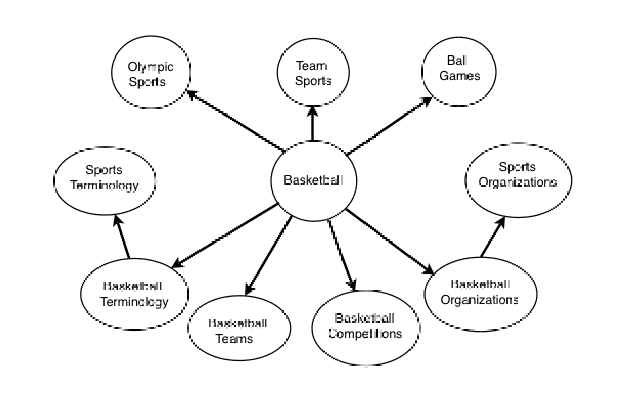
\includegraphics[width=90mm]{abbrv_bb_blanket.eps}
\caption{Abbreviated Markov blanket for the category Basketball}
\label{fig:abbrv_bb_blanket}
\end{figure}

The subcategories of the category Basketball (... Basketball Organizations, Basketball Competitions, Basketball Terminology, Basketball Teams...) can be seen as grabbing information specifc to the category. The supercategories (Ball Games, Olympic Sports, Team Sports) place the category in a higher perspective, abstractly describing basketball as a concept. The spousal categories are an abstract description of the subcategories.

Clustering the categories alone does not guarantee adequate corpus creation. Since the above model relies on the subcategories to describe specifcs of a given category, the ideal situation would be that the subcategories have many more pages than the supercategories and that there is a signifcant amount of information per page. In the case of Wikipedia, there are an average of 25.7 pages per category \cite{1321474}. The assumption for collecting the training data is the more subcategory data we have, the more detailed our description of our category. Considering that there are many categories that have much more than 26 pages, we instituted a PlusOne mechanism to extract extra information. This mechanism checks if a subcategory has an adequate number of pages a to fully describe its subtopic. We set this number to 10 * average, or 39. level represents how many extra levels we are to go down in the hierarchy, if necessary. SubjectSet is the overall set of all pages associated with the blanket structure along with any plusOne subjects obtained.


The overall mechanism does not take into account the amount of information within each page, but generally that can be ignored when considering the size of the blanket corpus when we extract the text from the Wikipedia subject pages. Using this method on the category Basketball, we can construct a corpus of 1843 subject pages and 1,301,006 terms.

When a category's corpus is built, we then build our n-gram frequency distributions and store them in a database for the NLP processing.


\section{Building Query Store}
\subsection{Query Resolution Recorder}
% Chris
Answering a question using the deep web requires one to navigate through a sequence of one or more web pages and links.  Many of the accesses involve clicks through web forms to resulting pages.  We have developed a model that represents the various actions a user may carry out during this process.  We record the user actions with a browser plugin called the \emph{query resolution recorder} (QRR).

During the answer retrieval process, a user discovers an element of the query's result on a web page.  Next, she highlights that element, typically a text string.  This highlight allows the QRR to record the source of  the query's answer.  The QRR stores all information from the user query in our data store.  When the user submits a web form she may associate each of the form's inputs with one of our stored context classes. 

The discovery process can be broken down into three cases:
\begin{enumerate}
\item The user typed in a URL  and highlighted part of or all the answer. 
\item The user typed in a URL, clicked a link, and found part or all of the answer. 
\item The user typed in a URL, filled out a form, and found part or all of the answer on a subsequent page. 
\end{enumerate}

Any discovery process  consists of a sequence of these transactions.  Additionally, data collected for inputs and outputs may be found during any stage of the complete discovery process.  An output collected during one stage of an extraction may be the input to a subsequent stage in the extraction.  The QRR builds the completed user collection process into a QRM.  The following is a mathematical formulation of information collected for user web interactions.\\

A QRM is a 5-tuple $Z = \left< \Upsilon, \Omega, P, M, R, A \right>$ such that:

\begin{enumerate}

\item $\Upsilon$ is the sequence of input classes $\left< \Upsilon_{1}, \Upsilon_{2}, \Upsilon_{3}, \Upsilon_{4} \right>$ where $\Upsilon_{1}$ represents the \emph{who} context of the associated query, $\Upsilon_{2}$ represents the \emph{what} context, $\Upsilon_{3}$ represents the \emph{when} context, and $\Upsilon_{4}$ represents the \emph{where} context.

\item $\Omega$ is the sequence of output classes $\left<\Omega_{1}, \Omega_{2}, \Omega_{3}, \Omega_{4}\right>$ where $\Omega_{1}$ represents the \emph{who} context of the associated query, $\Omega_{2}$ represents the \emph{what} context, $\Omega_{3}$ represents the \emph{when} context, and $\Omega_{4}$ represents the \emph{where} context.

\item $P$ is an ordered list of web pages $P = \left<P_1,P_2,..., P_n\right>$ where $P_h = \left<U_h,\left<I_{h_1},I_{h_2},...,I_{h_u}\right>,\left<O_{h_1},O_{h_2},...O_{h_v}\right>\right>$ for $1 \leq h \leq n$, $u = \left| I_h \right|$, $v = \left| O_h \right|$. $P_h$ is a triple comprised of a URL $U_h$, a sequence of input arguments, and a sequence of output results.
\\
Let $I_{\$} = \bigcup_{j=1}^{4} I_{\downarrow_j}$ be the set of the selector expressions for the inputs of a query and $O_{\$} = \bigcup_{j=1}^{4} O_{\downarrow_j}$ be the set of selectors expressions for the outputs of a query.
\\
Let $K$ be the set of all string constants.
\begin{itemize}
\item URI $U_1 \in K$ is a string and \\
for $1 < g \leq n$, URI $U_g \in K \cup \left( \bigcup^{g-1}_{p=1} \left( \bigcup^{\left|O_p\right|}_{h=1}O_{p_h} \right)\right)$ where $1 \leq h \leq \left| O_p \right| $,

\item for $1 < h < \left| I_1 \right|$, input $I_{1_h} \in K \cup I_{\$} \cup O_{\$}$ and \\
for $1 < g <= n$, then for $1 < h < \left| I_g \right|$, input $I_{g_h} \in K \cup I_{\$} \cup O_{\$} \cup \left( \bigcup^{g-1}_{p=1} \left( \bigcup^{\left|O_p\right|}_{h=1}O_{p_h} \right)\right)$.
\end{itemize}

\item $M$ is a map between $\Upsilon$, $K$, $\Omega$ to page list inputs $I_h$.

\item $R$ is an ontological realm. 

\item $A$ is the sequence of outputs from $\Upsilon$, $K$, and $\Omega$ representing the answer.

\end{enumerate}

%-------------------------------------------------------------------------------


\subsection{Generalization}
% Christan
The response pages created by querying web forms are dynamically generated with a templated structure. This generalization per page is done using the GenPath algorithm developed by Badica et al. \cite{Badica06}. Additionally, the community may be able to answer a particular SSQ using many different page interactions. Therefore, we proposed a method of generalizing extraction path to a result across pages. This method removes unnecessary page interactions and finds the shortest path to the result pages.

The websites that are wrapped are highly susceptible to structural changes \cite{TanZMG07}. Generalizing the extraction paths help to overcome small structural changes. If a website changes to the point where a QRM is no longer useful, the QRM not considered fresh. Morpheus allows users to rate the freshness of QRMs.

%-------------------------------------------------------------------------------


\section{Natural Language Queries}
\subsection{Semi-Structured Query}
% Joir-dan
\subsection{SSQ Ranking}
In order to match a new query with a SSQ within our data store, we have defined similarity measures between the ontologies of the new query and the candidate SSQs. These measures capture the distance between the ontology classes, properties, and individuals at the conceptual level in addition to simply matching URIs. The similarity measures are implemented in two scenarios: \textit{on-line execution} and \textit{off-line mode}. The \textit{on-line execution} is time sensitive and is used primarily for relating newly defined SSQs to the SSQs in the store. During \textit{off-line execution}, the system clusters similar SSQs.

The similarity measure for the SSQ ontologies is determined by the following components.
\begin{enumerate}
    \item QueryClass: an OWL class and the root of the SSQ ontology structure.
    \item hasRealm: an OWL object property with its domain as the SSQ Query class and its range as a realm class.
    \item Contexts such as who, what, when, and where are OWL object properties, whose domains are the query classes and ranges are OWL classes. 
    \item SSQClass: an OWL class which is created from the components described above.
\end{enumerate}
Based on this ontology structure and the execution scenarios, we have created an algorithm for finding the matches between SSQ ontologies. It is based on class divergence, which is motivated by the concept of multiple dispatch in CLOS \cite{95411} and Dylan programming \cite{Dylan_MultipleInheritance} for generic function type matches. We consider the realm class and context property ranges for determining SSQ similarity. Subsections \ref{sec:ctd}, and \ref{sec:oqom} describe about this in detail.

%-------------------------------------------------------------------------------

\subsubsection{Class Divergence}
\label{sec:ctd}
We employ a measure of compatibility, which we call \textit{class divergence}, between a source class and a target class using the \textit{topological structure} of the context classes in the ontology. We write $S \prec T$ for the reflexive transitive closure of the superclass relation. Let $d(P,Q)$ represent the hop distance in the directed ontology inheritance graph from $P$ to $Q$. The divergence between a source and target class ranges from zero (for identical classes) to one (for incompatible classes).  Let $S$ be the source class, $T$ be the target class, and let $C$ be a common ancestor class of $S$ and $T$ minimizing $d(S,C) + d(T,C)$. The class divergence between $S$ and $T$, the unnormalized class dissimilarity, is defined as follows:

\begin{equation}
d_{class}(S, T) = \begin{cases}
0 & if S.{uri} \equiv T.{uri}\\
d(S, T) & if S \prec T\\
1 & if T \prec S\\
d(S,root) \\+ d(S,C) + d(T,C) & otherwise
\end{cases}
\end{equation}

We normalize $d_{class}(S, T)$ by dividing by three times the height of the ontology tree.

Note, if $S \prec T$ and $S \not\prec Q$ then $d_{class}(S,T) < d_{class}(S,Q)$,
that is, the divergence of a source class to a target ancestor class is smaller than the divergence of a source class to any class that is not an ancestor. This is an important property in determining the compatibility of classes for answering queries.  If a SSQ answers queries concerning an ancestor class, it is more relevant that a SSQ that answers queries from any non-ancestral class. 

% Algorithm 1: figure  
\begin{figure}[t]
\centering
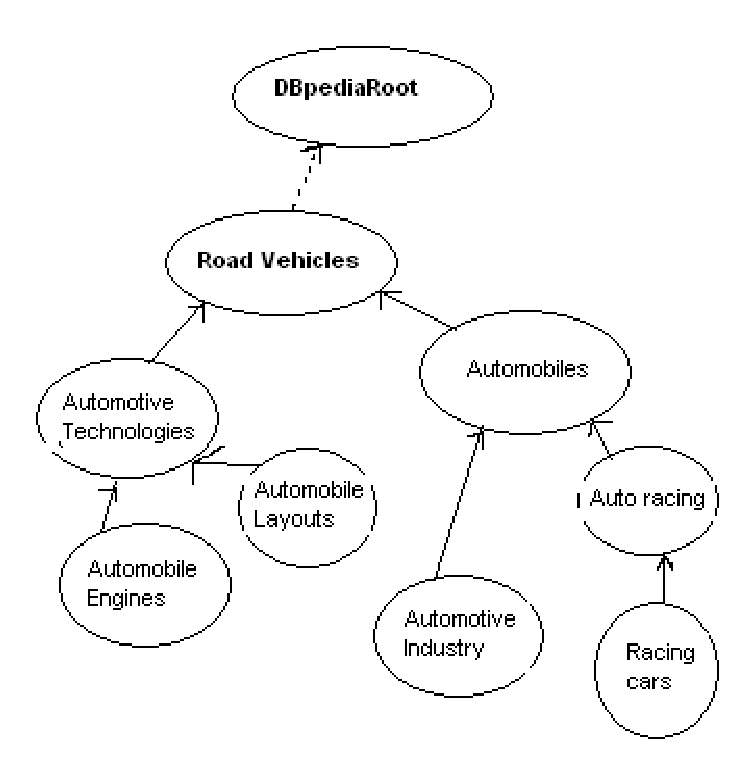
\includegraphics[width=90mm]{class_divergence.eps}
\caption{Abbrv. graphical representation of an automotive ontology}
\label{fig:class_divergence}
\end{figure}

Figure \ref{fig:class_divergence} illustrates the calculation of class divergence. This sample abbreviated ontology that was created from the DBpedia category heirarchy is rooted at the class \textit{DBpediaRoot}. The arrows represent the inheritance relationship between the classes in the topology. 

Suppose we want to find the divergence $d_{class}$\textit{(Automotive Industry, Racing Cars)}. The \textit{Automotive Industry} is the subclass of \textit{Automobiles} and \textit{Racing Cars} is the subclass of \textit{Auto Racinng}. Therefore, the common ancestor for these two can be determined as \textit{Automobiles} ($C$). They share the path from \textit{Automobiles} to the $root$. So, the unnormalized divergence \textit{d(Automotive Industry, root)} is 32 (calcuted from the path to root), \textit{d(Automotive Industry, Automobiles)} is one (dashed arrow), and \textit{d(Racing Cars, Automobiles)} is two (dashed arrow). Suppose, the ontology tree height is calculated as 294. Thus, \textit{d(Automotive Industry, Racing Cars)} is 35, which corresponds to a normalized value of $35/294$. 

%-------------------------------------------------------------------------------
\subsubsection{SSQ Ontology Matching}
\label{sec:oqom}

We use class divergence to calculate the relevance between a source SSQ and a target SSQ associated with a QRM.  Each SSQ will have four input classes, four output classes, and one realm.  We refer to the sequence of these classes $\langle \Upsilon_1, ..., \Upsilon_4, \Omega_1, ..., \Omega_4, R \rangle$ as the signature of an SSQ. If an input or output class is unspecified in the query, it is associated with the class $bottom$, which has no subclasses or individuals.

The relevance of QRM $Q$ with signature $\langle \Upsilon_{Q_1}, ..., \Upsilon_{Q_4}, \\\Omega_{Q_1}, ... , \Omega_{Q_4}, R_Q\rangle$ to SSQ $S$ with signature $\langle \Upsilon_{S_1}, ..., \Upsilon_{S_4}, \\\Omega_{S_1}, ... , \Omega_{S_4}, R_S \rangle$ is

\begin{eqnarray}
\label{qrmsimilarity}
 R(S,Q) = 1 - (d_{R} + d_{\Upsilon} + d_{\Omega})
\end{eqnarray}
\noindent where 
\begin{eqnarray}
d_{R} = \pi_9 d_{class}(R_S,R_Q) \nonumber
\end{eqnarray}
\begin{eqnarray}
d_{\Upsilon}  = \sum_{k=1}^4 {\pi_k} {d_{class}(\Upsilon_{S_k},\Upsilon_{Q_k})} \nonumber
\end{eqnarray}
\begin{eqnarray}
 d_{\Omega} = \sum_{j=1}^4 \pi_{4+j} d_{class}(\Omega_{S_j},\Omega_{Q_j})  \nonumber
\end{eqnarray}
\noindent the weights ${\pi}_k$ of the property hasRealm and other context properties satisfies the conditions 
\begin{equation}
\label{piconstraint1}
\sum_{k=1}^{9} {{\pi}_k} = 1
\end{equation}
\noindent and for $1 \leq i \leq 9$

\begin{equation}
\label{piconstraint2}
{\pi}_i > 0
\end{equation}

If an SSQ and a QRM have identical classes for all inputs and their realms then the QRM relevance value will be one. Otherwise, the relevance of the QRM will be in the range $[0, 1)$.   

% Need to show an example ?

%-------------------------------------------------------------------------------

\subsection{Query Re-Execution}
% Chris


\section{Results}
% Walk through of example query

\section{Future Work}
% Talk about the offline execution mode and class structural matching algorithm  

% Sort classes based on the prior 

\section{Conclusion}

\section{Acknowledgements}


%
% The bibliography for the citations in the paper 
\bibliographystyle{abbrv}
\bibliography{citations}  						% citations.bib is the name of the Bibliography


\end{document}            						% End of document. 
